\def\V{\text{\sc Vrai}\,}
\def\F{\text{\sc Faux}\,}
\def\ite{\text{\sc ite}\,}
%-------------------------------------------------------------------------------
%-------------------------------------------------------------------------------
\chapter{Mini Langage}
%-------------------------------------------------------------------------------
%-------------------------------------------------------------------------------
\thispagestyle{empty}
%-------------------------------------------------------------------------------
%-------------------------------------------------------------------------------
Nous allons définir un langage simple qui permet de travailler avec des fonctions d'une variable entière. 

Ce langage sera défini par adjonctions successives d'objets.

\begin{enumerate}
  \item On commence par les expressions arithmétiques simples, que l'on pourra évaluer.
  \item On ajoute alors la notion de variable et d'environnement de ces variables ; la valeur d'une variable sera définie par une expression et les expression pourront utiliser une variable déjà définie.
  \item On introduit ensuite les fonctions : elles seront pensées comme pouvant associer une valeur à une valeur donnée en entrée, cette dernière sera le résultat d'une expression. Les expression pourront alors utiliser des fonctions déjà définies.
  \item La programmation est introduite par les conditionnelles \type{si ... alors ... sinon} qui permettent de définir des fonctions plus générales.
  \item On finit par la récursivité qui est le moyen de plus simple d'effectuer des répétitions.
\end{enumerate}

On omettra la partie difficile qui consiste à interpréter une commande en texte en un programme compréhensible par l'ordinateur : nous écrirons directement les programmes sous forme d'arbres. 

On généralise le type classique des expression sous forme d'arbre binaire :
\begin{lstlisting}
type op = Plus | Moins | Fois;;
type expr = Val of int  |Ope of expr*op*expr
\end{lstlisting}
en un type plus général dont les composantes seront définies petit à petit :
\begin{lstlisting}
type op = Plus | Moins | Fois;;
type expr = |Val of int  
            |Ope of expr*op*expr
            |Var of string           (* partie 2 *)
            |Fn of string*expr       (* partie 3 *)
            |Ite of expr*expr*expr;; (* partie 4 *)
\end{lstlisting}

Les fonctions dont le paramètre est une expression utiliseront un pattern-matching et traiteront les composantes non définies par une dernière ligne de la forme :
 \begin{lstlisting}
  |_ -> failwith "non encore utilisable"
\end{lstlisting}

%--------------------------------------------------------------------------
%--------------------------------------------------------------------------
\section{Opérations simples}
%--------------------------------------------------------------------------
%--------------------------------------------------------------------------
On définit (provisoirement) une expression par un arbre binaire :

Dans cette ne expression peut être :
\begin{itemize}
  \item une valeur entière, une constante, représentée par \type{Val k},
  \item une opération simple entre deux expression représentée par un arbre.  
\end{itemize}

Il permettent de représenter les opérations simples ; par exemple 
\begin{lstlisting}
let e1 = Ope(Ope(Val 7,Moins,Val 3), 
             Fois, 
             Ope(Val 2,Plus,Val 4));;
\end{lstlisting}
représente $(7-3)*(2+4)$
%--------------------------------------------------------------------------
%--------------------------------------------------------------------------
\begin{Exercise}\it
Représenter $11 - (2 * (8-3))$.
\end{Exercise}
%--------------------------------------------------------------------------
\begin{Answer}
\begin{lstlisting}
let e2 = Ope (Val 11,
                Moins,
                Ope(Val 2,
                      Fois,
                      Ope(Val 8, Moins, Val 3)
                     )
               );;
\end{lstlisting} 
\end{Answer}
%--------------------------------------------------------------------------
%--------------------------------------------------------------------------
\begin{Exercise}\it
Écrire une fonction \type{eval} telle que \type{eval t} détermine la valeur de l'expression \type{t}.
\end{Exercise}
%--------------------------------------------------------------------------
\begin{Answer}
\begin{lstlisting}
let rec eval e =
  match e with
  |Val n -> n
  |Ope(e1, Plus, e2)  ->  eval e1 + eval e2
  |Ope(e1, Moins, e2) ->  eval e1 - eval e2
  |Ope(e1, Fois, e2)  ->  eval e1 * eval e2;;
\end{lstlisting} 
\end{Answer}
%--------------------------------------------------------------------------
\begin{lstlisting}
eval : expr -> int = <fun>
\end{lstlisting}
%--------------------------------------------------------------------------
\section{Variables}
%--------------------------------------------------------------------------
%--------------------------------------------------------------------------
On va maintenant incorporer les variables dans nos expressions.

Les variables sont des valeurs "à définir", représentées par une chaîne de caractères.

L'expression $(7-3)*(2+y)$ sera donc représentée par
\begin{lstlisting}
let e3 = Ope(Ope(Val 7, Moins, Val 3), 
             Fois, 
             Ope(Val 2, Plus, Var "y")
            );;
\end{lstlisting}

Les valeurs possibles des variables sont définies par une liste d'environnement dont les éléments sont des couples formés d'un nom de variable (\type{string}) et d'une valeur (\type{int}). 

Un environnement est donc un dictionnaire de type \type{(string*int) list}.
Par exemple, 
\begin{lstlisting}
let env0 = [("x",3); ("y",2)];;
\end{lstlisting}
 définit un environnement dans lequel 2 variables sont définies.
%--------------------------------------------------------------------------
%--------------------------------------------------------------------------
\begin{Exercise}\it 
Écrire une fonction \type{valeur} telle que \type{valeur var env} renvoie l'entier associé à la {\bf première apparition} de la variable \type{var} dans la liste \type{env}.
\end{Exercise}
%--------------------------------------------------------------------------
Par exemple \type{valeur "x" env} doit renvoyer 3.
%--------------------------------------------------------------------------
\begin{Answer}
\begin{lstlisting}
let rec valeur var env =
  match env with
  |[] -> failwith "Variable non liee"
  |(v, n)::reste when v = var -> n
  |c::reste -> valeur var l;;
\end{lstlisting} 
\end{Answer}
%--------------------------------------------------------------------------
\begin{lstlisting}
valeur : 'a -> ('a * 'b) list -> 'b = <fun>
\end{lstlisting}
%--------------------------------------------------------------------------
%--------------------------------------------------------------------------
\medskip

Pour ajouter une variable à un environnement on ajoute le couple \type{(nom, valeur)} en tête de l'environnement pour produire un nouvel environnement. On fait de même pour changer la valeur d'une variable : comme la valeur retournée est la première trouvée, on aura ainsi le bon résultat. Cela peut engendrer de nombreuses variables redondantes mais cela permet aussi de créer facilement des valeurs locales aux variables.
%--------------------------------------------------------------------------
%--------------------------------------------------------------------------
\begin{Exercise}\it
Écrire une fonction \type{eval2} 
telle que \type{eval2 t env} détermine la valeur de l'expression \type{t} dans l'environnement \type{env}.
\end{Exercise}
%--------------------------------------------------------------------------
\begin{Answer}
\begin{lstlisting}
let rec eval2 e env =
  match e with
  |Val n -> n
  |Var ch -> valeur ch env
  |Ope(e1, Plus, e2)  ->  eval2 e1 env + eval2 e2 env
  |Ope(e1, Moins, e2) ->  eval2 e1 env - eval2 e2 env
  |Ope(e1, Fois, e2)  ->  eval2 e1 env * eval2 e2 env;;
\end{lstlisting} 
\end{Answer}
%--------------------------------------------------------------------------
\begin{lstlisting}
eval2 : expr -> (string * int) list -> int = <fun>
\end{lstlisting}
%--------------------------------------------------------------------------
\medskip

Par exemple l'évaluation de \type{e3} avec l'environnement ci-dessus donne 16
%--------------------------------------------------------------------------
\newpage
%--------------------------------------------------------------------------
\section{Fonctions}
%--------------------------------------------------------------------------
%--------------------------------------------------------------------------
On se restreint aux fonctions d'une variable.

Une fonction est définie par un triplet \type{("f", "x", expF)} où \type{expF} est une expression. La valeur de \type{f} en \type{k} est obtenue en donnant à la variable \type{x} la valeur \type{k} dans \type{expF}.

Par exemple, si \type{c = Ope(Var "x", Fois, Var "x")}, le triplet \type{("f", "x", c)} représente la fonction carré.

Les fonctions sont gérées par une liste de fonctions. Par exemple
\begin{lstlisting}
let fonc0 = [("f", "x", Ope(Val 2, Fois, Var "x")); 
             ("g", "x", Ope(Var "x", Plus, Val 1))];;
\end{lstlisting}

Un environnement de fonctions est donc un dictionnaire (généralisé) de type 

\type{(string * string * expr) list}.
%--------------------------------------------------------------------------
%--------------------------------------------------------------------------
\begin{Exercise}\it
Écrire une fonction \type{defin} 
telle que \type{defin f fonc} renvoie le nom de la variable (une chaîne de caractères) et l'expression associés à une fonction de nom \type{f} dans la liste de fonctions.
\end{Exercise}
%--------------------------------------------------------------------------
\begin{Answer}
\begin{lstlisting}
let rec defin f fonc =
  match fonc with
  |[] -> failwith "Fonction non liee"
  |(fn, var, exp)::_ when fn = f -> (var,exp)
  |_::reste -> defin f reste;;
\end{lstlisting} 
\end{Answer}
%--------------------------------------------------------------------------
\begin{lstlisting}
defin : 'a -> ('a * 'b * 'c) list -> 'b * 'c = <fun>
\end{lstlisting}
%--------------------------------------------------------------------------
\medskip

On utilise donc le constructeur \type{Fn} dans les expression.

Les paramètres sont une chaîne de caractères, le nom de la fonction, et une expression \type{expV}. 

Le résultat de l'expression \type{expV} sera la valeur envoyée à $f$.

Par exemple, avec l'environnement de fonctions ci-dessus,

\type{Fn("f", Ope(Val 7, Moins, Var "x"))} sera évalué en $8$.

On notera que $x$ est associé à 3 lors du calcul de \type{Ope(Val 7, Moins, Var "x"))} 

mais qu'il prend la valeur 4 lors de l'évaluation de $f$

%--------------------------------------------------------------------------
\begin{Exercise}\it
Écrire une fonction \type{eval3} telle que \type{eval t env fonc} détermine la valeur de l'expression \type{t} dans l'environnement \type{env} avec les fonctions de \type{fonc}.
\end{Exercise}
%--------------------------------------------------------------------------
\begin{Answer}
\begin{lstlisting}
let rec eval3 t env fonc =
  match t with
  |Val n -> n
  |Var ch -> valeur ch env
  |Ope(t1, Plus, t2)  ->  eval3 t1 env fonc + eval3 t2 env fonc
  |Ope(t1, Moins, t2) ->  eval3 t1 env fonc - eval3 t2 env fonc
  |Ope(t1, Fois, t2)  ->  eval3 t1 env fonc * eval3 t2 env fonc
  |Fn(f, expV) -> let var, expF = defin f fonc in
                  let env1 = (var, eval expV env fonc)::env in
                  eval3 expF env1 fonc;;
\end{lstlisting} 
\end{Answer}
%-------------------------------------------------------------------------- de signature
\begin{lstlisting}
eval3 : expr  -> (string * int) list 
              -> (string * string * expr) list 
              -> int = <fun>
\end{lstlisting}
%--------------------------------------------------------------------------
\medskip
Exemple
\begin{lstlisting}
let e4 = Ope(Fn("f", Ope(Val 7, Moins,Val 3)),
               Fois,
               Ope(Val 2, Plus, Var "y"));;

eval3 e4 env0 fonc0;;

- : int = 32
\end{lstlisting}
%--------------------------------------------------------------------------
\newpage
%--------------------------------------------------------------------------
\section{Condionnelles}
%--------------------------------------------------------------------------
%--------------------------------------------------------------------------
On peut définir une instruction de branchement par un arbre 
\[
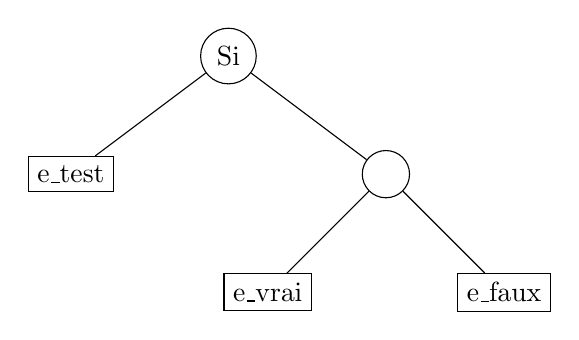
\begin{tikzpicture}[level distance =15mm]
  \tikzstyle{level 1}=[sibling distance =4cm]
  \tikzstyle{level 2}=[sibling distance =3cm]
  \tikzstyle{level 3}=[sibling distance =2cm]
  \tikzstyle{every node}=[draw]
  \node[circle] {\type{Si}}
   child {node{\type{e\_test}}}
  child {node[circle, minimum size = 6mm]{}
           child {node{\type{e\_vrai}}}
           child {node{\type{e\_faux}}}
        };
\end{tikzpicture}
\]

où \type{e\_test}, \type{e\_vrai} et \type{e\_faux} sont des expressions.

Si \type{e\_test} est évaluée à une valeur $n$ avec $n > 0$ alors le résultat est l'évaluation de \type{e\_vrai}, sinon le résultat est l'évaluation de \type{e\_faux}.

On utilise donc le dernier constructeur : \type{Ite}.

L'arbre ci-dessus sera codé \type{Ite(e\_test, e\_vrai, e\_faux)}.
%--------------------------------------------------------------------------
%--------------------------------------------------------------------------
\begin{Exercise}\it
Écrire une fonction \type{signe x} sous forme d'un triplet \type{("signe", "x", e\_signe)} qui renvoie 1 pour $x > 0$, $-1$ pour $x < 0$ et 0 si $x$ est nul.
\end{Exercise}
%--------------------------------------------------------------------------
\begin{Answer}
\begin{lstlisting}
e_signe = Ite(Var "x", Val 1, Ite(Ope(Val 0, Moins, Var "x"), Val (-1), Val 0))      
\end{lstlisting} 
\end{Answer}
%--------------------------------------------------------------------------
%--------------------------------------------------------------------------
\begin{Exercise}\it
Modifier la fonction d'évaluation en \type{eval4} pour tenir compte de cet opérateur.
\end{Exercise}
%--------------------------------------------------------------------------
\begin{Answer}
\begin{lstlisting}
let rec eval4 e env fonc =
  match e with
  |Val(n) -> n
  |Var(v) -> valeur v env
  |Ope(e1, Plus, e2)  ->  eval4 e1 env fonc + eval4 e2 env fonc
  |Ope(e1, Moins, e2) ->  eval4 e1 env fonc - eval4 e2 env fonc
  |Ope(e1, Fois, e2)  ->  eval4 e1 env fonc * eval4 e2 env fonc
  |Fn(f, expV) -> let v, expF = defin f fonc in
                  let env1 = (v, eval4 expV env fonc)::env in
                  eval4 expF env1 fonc
  |Ite(eT, eV, eF) -> if eval4 eT env fonc > 0
                      then eval4 eV env fonc
                      else eval4 eF env fonc;;
\end{lstlisting} 
\end{Answer}
\bigskip

On peut alors introduire des fonctions récursives, une conditionnelle permettant de gérer le cas d'arrêt.
%--------------------------------------------------------------------------
%--------------------------------------------------------------------------
\begin{Exercise}\it
Écrire la fonction factorielle.
\end{Exercise}
%--------------------------------------------------------------------------
\begin{Answer}
\begin{lstlisting}
let e_boucle = Ope(Var "n", Fois, Fn("fact", Ope(Var "n", Moins, Val 1)));;
                  
let e_fact = Ite(Var "n", e_boucle, Val 1);;

let fonc1 = ("fact", "n", e_fact)::fonc0;;
\end{lstlisting} 
\end{Answer}
%--------------------------------------------------------------------------
%--------------------------------------------------------------------------


